%!TEX ROOT=formularioFisica.tex

\section{Idrostatica}
L'idrostatica studia i fluidi in stato di equilibrio. Studia anche le pressioni.
\subsection{Legge di Stevino}
La legge di Stevino permette di trovare la pressione ad una data profondità.
\begin{equation*}
  \Delta p = \delta gh
\end{equation*}
$\delta$: densità del liquido\\
\hyperref[tab:patm]{$p_{atm}$}: $1\,\text{atm} = 1.01\cdot10^5\,\text{Pa} = 760\,\text{mm\,Hg} = 
1.01\cdot10^5\,\text{N/m}^2 = 1\,\text{bar}$\\
\hyperref[tab:g]{$g$}: $9.81\,\text{m/s}^2$\\
$h$: profondità\\[\baselineskip]
Se vista in un modo più generale si trova la pressione tra due punti
\begin{equation*}
  p_2 = p_1 + \delta g\Delta h
\end{equation*}
\begin{center}
  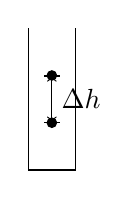
\begin{tikzpicture}[scale=0.6]
    \draw (0,0) -- ++(0,-3) -- ++(1,0) -- ++(0,3);
    \filldraw (0.5,-1) circle (0.1);
    \filldraw (0.5,-2) circle (0.1);
    \draw[|<->|] (0.5,-1) -- (0.5,-2)
      node[pos=0.5,right]{$\Delta h$};
  \end{tikzpicture}
\end{center}

$\delta$: densità del liquido\\
\hyperref[tab:g]{$g$}: $9.81\,\text{m/s}^2$\\
$h$: profondità\\ [\baselineskip]

Si ricordi che $\text{Densità}=\frac{\text{Massa}}{\text{Volume}}$.

\subsection{Torchio idraulico}
\begin{center}
  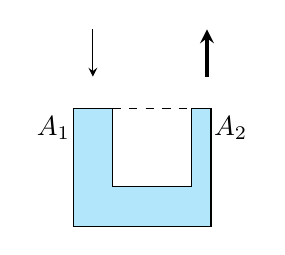
\begin{tikzpicture}
    \filldraw[cyan, fill opacity = 0.3]
      (0,0) -- ++(0.5,0) -- ++(0,-1) -- ++(1,0) -- ++(0,1) -- ++(0.25,0) --
      ++(0,-1.5) -- ++(-1.75,0) -- ++(0,1.5);
    \draw 
      (0,0) -- ++(0.5,0) -- ++(0,-1) -- ++(1,0) -- ++(0,1) -- ++(0.25,0) --
      ++(0,-1.5) -- ++(-1.75,0) -- ++(0,1.5);
    \draw[dashed] (0.5,0) -- +(1,0);
    \node at (0-.25,-0.25){$A_1$};
    \draw[stealth-] (0.25, 0.4) -- ++(0,0.6);
    \node at (2,-0.25){$A_2$};
    \draw[-stealth,very thick] (1.7,0.4) -- ++(0,0.6);
  \end{tikzpicture}
\end{center}
Il torchio idraulico permette partendo da una forza applicata su un pistone (di area $A_1$) di ottenere
una forza più grande su un altro pistone (di area $A_2$).
\begin{equation*}
  p = \frac{F}{A}\qquad \frac{F_1}{A_1}=\frac{F_2}{A_2}
\end{equation*}

\subsection{Principio di Pascal}
Il principio di Pascal afferma che in un liquido  una pressione che venga esercitata in un punto  
viene trasmessa a ogni suo altro punto e in ogni sua direzione.
\begin{center}
  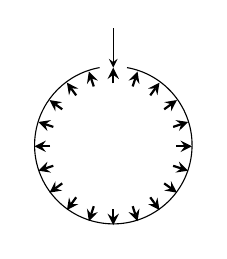
\begin{tikzpicture}
    \draw ++(0.175,1) arc(80:-260:1);
    \draw[-stealth] (0,1.5) -- ++(0,-0.5);
    \foreach \x in {1,...,20}{\draw[thick,-stealth] 
      ({\x*360/20}:0.8cm) -- ++({\x*360/20}:0.2cm);}
    \end{tikzpicture}
  \end{center}

  \subsection{Manometro ad U}
  Se un tubo viene riempito con due liquidi di densità diversa, l'altezza misurata a destra e 
  sinistra sarà diversa.
  \begin{center}
    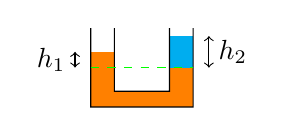
\begin{tikzpicture}
      \coordinate (H1a) at (0,0.5);
      \coordinate (H1b) at (0.3,0.7);
      \coordinate (H2a) at (1,0.5);
      \coordinate (H2b) at (1.3,0.9);
      \fill[orange] (0,0) -- (0.3,0) -- (0.3,0.7) -- (0,0.7) -- cycle;
      \fill[orange] (0,0) -- (1.3,0) -- (1.3,0.2) -- (0,0.2) -- cycle;
      \fill[orange] (1.3,0) -- (1.3,0.5) -- (1,0.5) -- (1,0) -- cycle;
      \fill[cyan] (H2a) -- ++(0.3,0) -- (H2b) -- ++(-0.3,0) -- cycle;
      \draw (H1a) -| (0,1) -- ++(0,-1) -- ++(1.3,0) -- (1.3,1)  ++(-0.3,0) -- ++(0,-0.8) --
        ++(-0.7,0) -- (0.3,1);
      \draw [dashed,green](0,0.5)--(1.3,0.5);
      \draw[<->] (-0.2,0.5) -- ++(0,0.2)
        node[pos=0.5,left]{$h_1$};
      \draw[<->] (1.5,0.5) -- ++(0,0.4)
        node[pos=0.5,right]{$h_2$};
    \end{tikzpicture}
  \end{center}
  \begin{equation*}
    \frac{h_1}{h_2} = \frac{\delta_2}{\delta_1}
  \end{equation*}
  Si presti attenzione alla densità corretta e all'$h$ corretto.

  \subsection{Principio di Archimede}
  Il principio di Archimede permette di trovare la forza di galleggiamento.\\
  Il principio di Archimede stabilisce che un corpo immerso in un liquido o in un gas (come l'aria) 
  riceve una spinta dal basso verso l'alto.
  \begin{equation*}
    F_g = \delta_fVg
  \end{equation*}
  Al principio di Archimede è collegata la condizione di equilibrio di un corpo in un fluido:\\
  \begin{center}
    \emph{`Un corpo è in equilibrio in un fluido se la sua forza peso compensa la spinta di 
    Archimede, cioè se il suo peso è uguale al peso del fluido spostato.'}
  \end{center}

  \subsection{Volume della parte immersa}
  \begin{equation*}
    V_{imm} = V_{tot}\frac{\delta_s}{\delta_f}
  \end{equation*}
  $\delta_s$: densità del corpo\\
  $\delta_f$: densità del fluido\\
  $V_{tot}$: volume del corpo

  \begin{center}
    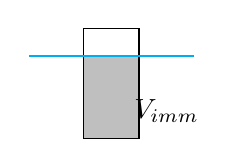
\begin{tikzpicture}[scale=0.7]
      \fill[gray!50] (0,1.5) -- ++(1,0) -- ++(0,-1.5) -- ++(-1,0) -- cycle;
      \draw (0,0) -- ++(1,0) -- ++(0,2) -- ++(-1,0) -- cycle;
      \draw[cyan,thick] (-1,1.5) -- ++(3,0);

      \node at (1.5,0.5){$V_{imm}$};
    \end{tikzpicture}
  \end{center}
